\documentclass[../main.tex]{subfiles}

\begin{document}
\chapter{前言}

\begin{center}
  \emph{“把丢失的初高中计算机基础知识和大学丢失的开发能力补回来”}
\end{center}

计算机基础科学教育是我国近些年一直努力推进的教育之一,北京大学的所有学生都应修习《计算概论》课程。然而,大学计算机基础教育的内容往往过于理论化,缺乏实用性,这使得同学们在学习过程中容易感到枯燥乏味,在学习之后也很难将所学知识灵活应用到实际生产与生活中,最终导致在校学生对计算机的使用和开发能力普遍较低,甚至出现了“念了四年本科却不会用Git”的现象。。同时,我国初高中乃至小学阶段,计算机的教育水平参差不齐,同学们的基础也不尽相同,这导致部分基础较差的同学在学习《计算概论》时会遇到困难,遑论进阶课程。

在本手册正式编写之前,已经有很多学长为了抹平基础知识的差距做出了相关的努力。几个广为人知的项目:北京大学为新生提供了《计算概论衔接课》,旨在帮助同学们快速入门计算机基础知识(这门课的前半部分由我所讲授);北京大学学生Linux俱乐部(LCPU)启动了Getting Started项目,旨在帮助同学们快速入门Linux和计算机科学(该项目亦由我全权负责);一位\faGithub\href{https://github.com/PKUFlyingPig}{学长}发起了\href{https://csdiy.wiki/}{CS自学指南}项目,受到了广泛的关注和认可,该项目迄今已有一百五十余位贡献者;PKUHub等其他官方或非官方的组织也在积极推动计算机基础教育的普及。

然而,Getting Started和自学指南对于大一新生而言,存在的最大不足之处就是:不够基础。而对于有能力就读北大的学生而言,“上课”这种获取信息的形式的信息密度显然是不够的,大约是已经不再幻想上课有用了;真正有用的知识还是要靠同学们自己去学习实践。因此,我认为给同学们一本手册要比给同学们数小时的课程视频有用得多。笔者最终决定:制作这份手册,帮助同学们把初高中缺失的计算机知识,以及大学丢失的开发能力补回来。

本手册可以认为是对大学常用计算机基础知识与基础开发能力的汇总,比起深度更注重广度,比起理论更注重实践。简而言之,我们手册中会讲一些\textbf{正课几乎不会讲、但是用处极大}的知识。我们认为使用本手册的同学都已经具备了最基本的计算机操作能力,例如“使用鼠标”“关机”这种操作,因此也不会涉及相关内容。

本手册正文分为两部分。第一部分面向计算机新手,讲述计算机基础知识,内容涵盖计算机组成和使用、编程环境配置、文本处理、Linux等内容,旨在将同学们的水平提升至能够接受大学计算机基础教育的水平;第二部分则面向工程开发新手,讲述工程开发的一些基础内容,涵盖了实用主义编程、调试和C语言工具链等,旨在将同学们的水平提升至能够进行简单工程开发的水平。两部分内容均以实用为主,力求让同学们能够学以致用。当然,一点理论知识都不会的同学阅读本手册显然是有困难的,为了解决这些问题,笔者也在本手册的末尾增加了一些附录,来非常粗浅地解释一些理论知识。

本手册以本人实践和经验为基底讲授。\textbf{如果本手册中的内容和正课中的内容或要求有差异,请以正课为准。}

本手册参考了\href{https://missing.lcpu.dev}{LCPU Getting Started}以及诸多博文、指南的内容,并在此基础上进行了增删和修改。

希望本手册能够对同学们有所帮助。

如有疑问,欢迎来我的GitHub主页(\faGithub\href{https://github.com/ZangXuanyi/getting-started-handout}{ZangXuanyi/getting-started-handout})查看本手册的源代码,并提出Issue与Pull Request。如不能访问,也可向我发送电子邮件咨询:\texttt{zangxuanyi@stu.pku.edu.cn}。

\begin{figure}[ht]
  \centering
  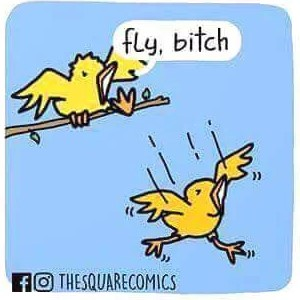
\includegraphics[width=0.5\textwidth]{images/fly.jpg}
\end{figure}



\end{document}